\documentclass[11pt]{article}

    \usepackage[breakable]{tcolorbox}
    \usepackage{parskip} % Stop auto-indenting (to mimic markdown behaviour)
    
    \usepackage{iftex}
    \ifPDFTeX
    	\usepackage[T1]{fontenc}
    	\usepackage{mathpazo}
    \else
    	\usepackage{fontspec}
    \fi

    % Basic figure setup, for now with no caption control since it's done
    % automatically by Pandoc (which extracts ![](path) syntax from Markdown).
    \usepackage{graphicx}
    % Maintain compatibility with old templates. Remove in nbconvert 6.0
    \let\Oldincludegraphics\includegraphics
    % Ensure that by default, figures have no caption (until we provide a
    % proper Figure object with a Caption API and a way to capture that
    % in the conversion process - todo).
    \usepackage{caption}
    \DeclareCaptionFormat{nocaption}{}
    \captionsetup{format=nocaption,aboveskip=0pt,belowskip=0pt}

    \usepackage{float}
    \floatplacement{figure}{H} % forces figures to be placed at the correct location
    \usepackage{xcolor} % Allow colors to be defined
    \usepackage{enumerate} % Needed for markdown enumerations to work
    \usepackage{geometry} % Used to adjust the document margins
    \usepackage{amsmath} % Equations
    \usepackage{amssymb} % Equations
    \usepackage{textcomp} % defines textquotesingle
    % Hack from http://tex.stackexchange.com/a/47451/13684:
    \AtBeginDocument{%
        \def\PYZsq{\textquotesingle}% Upright quotes in Pygmentized code
    }
    \usepackage{upquote} % Upright quotes for verbatim code
    \usepackage{eurosym} % defines \euro
    \usepackage[mathletters]{ucs} % Extended unicode (utf-8) support
    \usepackage{fancyvrb} % verbatim replacement that allows latex
    \usepackage{grffile} % extends the file name processing of package graphics 
                         % to support a larger range
    \makeatletter % fix for old versions of grffile with XeLaTeX
    \@ifpackagelater{grffile}{2019/11/01}
    {
      % Do nothing on new versions
    }
    {
      \def\Gread@@xetex#1{%
        \IfFileExists{"\Gin@base".bb}%
        {\Gread@eps{\Gin@base.bb}}%
        {\Gread@@xetex@aux#1}%
      }
    }
    \makeatother
    \usepackage[Export]{adjustbox} % Used to constrain images to a maximum size
    \adjustboxset{max size={0.9\linewidth}{0.9\paperheight}}

    % The hyperref package gives us a pdf with properly built
    % internal navigation ('pdf bookmarks' for the table of contents,
    % internal cross-reference links, web links for URLs, etc.)
    \usepackage{hyperref}
    % The default LaTeX title has an obnoxious amount of whitespace. By default,
    % titling removes some of it. It also provides customization options.
    \usepackage{titling}
    \usepackage{longtable} % longtable support required by pandoc >1.10
    \usepackage{booktabs}  % table support for pandoc > 1.12.2
    \usepackage[inline]{enumitem} % IRkernel/repr support (it uses the enumerate* environment)
    \usepackage[normalem]{ulem} % ulem is needed to support strikethroughs (\sout)
                                % normalem makes italics be italics, not underlines
    \usepackage{mathrsfs}
    

    
    % Colors for the hyperref package
    \definecolor{urlcolor}{rgb}{0,.145,.698}
    \definecolor{linkcolor}{rgb}{.71,0.21,0.01}
    \definecolor{citecolor}{rgb}{.12,.54,.11}

    % ANSI colors
    \definecolor{ansi-black}{HTML}{3E424D}
    \definecolor{ansi-black-intense}{HTML}{282C36}
    \definecolor{ansi-red}{HTML}{E75C58}
    \definecolor{ansi-red-intense}{HTML}{B22B31}
    \definecolor{ansi-green}{HTML}{00A250}
    \definecolor{ansi-green-intense}{HTML}{007427}
    \definecolor{ansi-yellow}{HTML}{DDB62B}
    \definecolor{ansi-yellow-intense}{HTML}{B27D12}
    \definecolor{ansi-blue}{HTML}{208FFB}
    \definecolor{ansi-blue-intense}{HTML}{0065CA}
    \definecolor{ansi-magenta}{HTML}{D160C4}
    \definecolor{ansi-magenta-intense}{HTML}{A03196}
    \definecolor{ansi-cyan}{HTML}{60C6C8}
    \definecolor{ansi-cyan-intense}{HTML}{258F8F}
    \definecolor{ansi-white}{HTML}{C5C1B4}
    \definecolor{ansi-white-intense}{HTML}{A1A6B2}
    \definecolor{ansi-default-inverse-fg}{HTML}{FFFFFF}
    \definecolor{ansi-default-inverse-bg}{HTML}{000000}

    % common color for the border for error outputs.
    \definecolor{outerrorbackground}{HTML}{FFDFDF}

    % commands and environments needed by pandoc snippets
    % extracted from the output of `pandoc -s`
    \providecommand{\tightlist}{%
      \setlength{\itemsep}{0pt}\setlength{\parskip}{0pt}}
    \DefineVerbatimEnvironment{Highlighting}{Verbatim}{commandchars=\\\{\}}
    % Add ',fontsize=\small' for more characters per line
    \newenvironment{Shaded}{}{}
    \newcommand{\KeywordTok}[1]{\textcolor[rgb]{0.00,0.44,0.13}{\textbf{{#1}}}}
    \newcommand{\DataTypeTok}[1]{\textcolor[rgb]{0.56,0.13,0.00}{{#1}}}
    \newcommand{\DecValTok}[1]{\textcolor[rgb]{0.25,0.63,0.44}{{#1}}}
    \newcommand{\BaseNTok}[1]{\textcolor[rgb]{0.25,0.63,0.44}{{#1}}}
    \newcommand{\FloatTok}[1]{\textcolor[rgb]{0.25,0.63,0.44}{{#1}}}
    \newcommand{\CharTok}[1]{\textcolor[rgb]{0.25,0.44,0.63}{{#1}}}
    \newcommand{\StringTok}[1]{\textcolor[rgb]{0.25,0.44,0.63}{{#1}}}
    \newcommand{\CommentTok}[1]{\textcolor[rgb]{0.38,0.63,0.69}{\textit{{#1}}}}
    \newcommand{\OtherTok}[1]{\textcolor[rgb]{0.00,0.44,0.13}{{#1}}}
    \newcommand{\AlertTok}[1]{\textcolor[rgb]{1.00,0.00,0.00}{\textbf{{#1}}}}
    \newcommand{\FunctionTok}[1]{\textcolor[rgb]{0.02,0.16,0.49}{{#1}}}
    \newcommand{\RegionMarkerTok}[1]{{#1}}
    \newcommand{\ErrorTok}[1]{\textcolor[rgb]{1.00,0.00,0.00}{\textbf{{#1}}}}
    \newcommand{\NormalTok}[1]{{#1}}
    
    % Additional commands for more recent versions of Pandoc
    \newcommand{\ConstantTok}[1]{\textcolor[rgb]{0.53,0.00,0.00}{{#1}}}
    \newcommand{\SpecialCharTok}[1]{\textcolor[rgb]{0.25,0.44,0.63}{{#1}}}
    \newcommand{\VerbatimStringTok}[1]{\textcolor[rgb]{0.25,0.44,0.63}{{#1}}}
    \newcommand{\SpecialStringTok}[1]{\textcolor[rgb]{0.73,0.40,0.53}{{#1}}}
    \newcommand{\ImportTok}[1]{{#1}}
    \newcommand{\DocumentationTok}[1]{\textcolor[rgb]{0.73,0.13,0.13}{\textit{{#1}}}}
    \newcommand{\AnnotationTok}[1]{\textcolor[rgb]{0.38,0.63,0.69}{\textbf{\textit{{#1}}}}}
    \newcommand{\CommentVarTok}[1]{\textcolor[rgb]{0.38,0.63,0.69}{\textbf{\textit{{#1}}}}}
    \newcommand{\VariableTok}[1]{\textcolor[rgb]{0.10,0.09,0.49}{{#1}}}
    \newcommand{\ControlFlowTok}[1]{\textcolor[rgb]{0.00,0.44,0.13}{\textbf{{#1}}}}
    \newcommand{\OperatorTok}[1]{\textcolor[rgb]{0.40,0.40,0.40}{{#1}}}
    \newcommand{\BuiltInTok}[1]{{#1}}
    \newcommand{\ExtensionTok}[1]{{#1}}
    \newcommand{\PreprocessorTok}[1]{\textcolor[rgb]{0.74,0.48,0.00}{{#1}}}
    \newcommand{\AttributeTok}[1]{\textcolor[rgb]{0.49,0.56,0.16}{{#1}}}
    \newcommand{\InformationTok}[1]{\textcolor[rgb]{0.38,0.63,0.69}{\textbf{\textit{{#1}}}}}
    \newcommand{\WarningTok}[1]{\textcolor[rgb]{0.38,0.63,0.69}{\textbf{\textit{{#1}}}}}
    
    
    % Define a nice break command that doesn't care if a line doesn't already
    % exist.
    \def\br{\hspace*{\fill} \\* }
    % Math Jax compatibility definitions
    \def\gt{>}
    \def\lt{<}
    \let\Oldtex\TeX
    \let\Oldlatex\LaTeX
    \renewcommand{\TeX}{\textrm{\Oldtex}}
    \renewcommand{\LaTeX}{\textrm{\Oldlatex}}
    % Document parameters
    % Document title
    \title{Formal Power Series in Macaulay2\\ \large REU Symposium Summer 2021}
    \author{Annie Giokas\\{ Advisor: Karl Schwede}}
    
    
    
    
% Pygments definitions
\makeatletter
\def\PY@reset{\let\PY@it=\relax \let\PY@bf=\relax%
    \let\PY@ul=\relax \let\PY@tc=\relax%
    \let\PY@bc=\relax \let\PY@ff=\relax}
\def\PY@tok#1{\csname PY@tok@#1\endcsname}
\def\PY@toks#1+{\ifx\relax#1\empty\else%
    \PY@tok{#1}\expandafter\PY@toks\fi}
\def\PY@do#1{\PY@bc{\PY@tc{\PY@ul{%
    \PY@it{\PY@bf{\PY@ff{#1}}}}}}}
\def\PY#1#2{\PY@reset\PY@toks#1+\relax+\PY@do{#2}}

\@namedef{PY@tok@w}{\def\PY@tc##1{\textcolor[rgb]{0.73,0.73,0.73}{##1}}}
\@namedef{PY@tok@c}{\let\PY@it=\textit\def\PY@tc##1{\textcolor[rgb]{0.25,0.50,0.50}{##1}}}
\@namedef{PY@tok@cp}{\def\PY@tc##1{\textcolor[rgb]{0.74,0.48,0.00}{##1}}}
\@namedef{PY@tok@k}{\let\PY@bf=\textbf\def\PY@tc##1{\textcolor[rgb]{0.00,0.50,0.00}{##1}}}
\@namedef{PY@tok@kp}{\def\PY@tc##1{\textcolor[rgb]{0.00,0.50,0.00}{##1}}}
\@namedef{PY@tok@kt}{\def\PY@tc##1{\textcolor[rgb]{0.69,0.00,0.25}{##1}}}
\@namedef{PY@tok@o}{\def\PY@tc##1{\textcolor[rgb]{0.40,0.40,0.40}{##1}}}
\@namedef{PY@tok@ow}{\let\PY@bf=\textbf\def\PY@tc##1{\textcolor[rgb]{0.67,0.13,1.00}{##1}}}
\@namedef{PY@tok@nb}{\def\PY@tc##1{\textcolor[rgb]{0.00,0.50,0.00}{##1}}}
\@namedef{PY@tok@nf}{\def\PY@tc##1{\textcolor[rgb]{0.00,0.00,1.00}{##1}}}
\@namedef{PY@tok@nc}{\let\PY@bf=\textbf\def\PY@tc##1{\textcolor[rgb]{0.00,0.00,1.00}{##1}}}
\@namedef{PY@tok@nn}{\let\PY@bf=\textbf\def\PY@tc##1{\textcolor[rgb]{0.00,0.00,1.00}{##1}}}
\@namedef{PY@tok@ne}{\let\PY@bf=\textbf\def\PY@tc##1{\textcolor[rgb]{0.82,0.25,0.23}{##1}}}
\@namedef{PY@tok@nv}{\def\PY@tc##1{\textcolor[rgb]{0.10,0.09,0.49}{##1}}}
\@namedef{PY@tok@no}{\def\PY@tc##1{\textcolor[rgb]{0.53,0.00,0.00}{##1}}}
\@namedef{PY@tok@nl}{\def\PY@tc##1{\textcolor[rgb]{0.63,0.63,0.00}{##1}}}
\@namedef{PY@tok@ni}{\let\PY@bf=\textbf\def\PY@tc##1{\textcolor[rgb]{0.60,0.60,0.60}{##1}}}
\@namedef{PY@tok@na}{\def\PY@tc##1{\textcolor[rgb]{0.49,0.56,0.16}{##1}}}
\@namedef{PY@tok@nt}{\let\PY@bf=\textbf\def\PY@tc##1{\textcolor[rgb]{0.00,0.50,0.00}{##1}}}
\@namedef{PY@tok@nd}{\def\PY@tc##1{\textcolor[rgb]{0.67,0.13,1.00}{##1}}}
\@namedef{PY@tok@s}{\def\PY@tc##1{\textcolor[rgb]{0.73,0.13,0.13}{##1}}}
\@namedef{PY@tok@sd}{\let\PY@it=\textit\def\PY@tc##1{\textcolor[rgb]{0.73,0.13,0.13}{##1}}}
\@namedef{PY@tok@si}{\let\PY@bf=\textbf\def\PY@tc##1{\textcolor[rgb]{0.73,0.40,0.53}{##1}}}
\@namedef{PY@tok@se}{\let\PY@bf=\textbf\def\PY@tc##1{\textcolor[rgb]{0.73,0.40,0.13}{##1}}}
\@namedef{PY@tok@sr}{\def\PY@tc##1{\textcolor[rgb]{0.73,0.40,0.53}{##1}}}
\@namedef{PY@tok@ss}{\def\PY@tc##1{\textcolor[rgb]{0.10,0.09,0.49}{##1}}}
\@namedef{PY@tok@sx}{\def\PY@tc##1{\textcolor[rgb]{0.00,0.50,0.00}{##1}}}
\@namedef{PY@tok@m}{\def\PY@tc##1{\textcolor[rgb]{0.40,0.40,0.40}{##1}}}
\@namedef{PY@tok@gh}{\let\PY@bf=\textbf\def\PY@tc##1{\textcolor[rgb]{0.00,0.00,0.50}{##1}}}
\@namedef{PY@tok@gu}{\let\PY@bf=\textbf\def\PY@tc##1{\textcolor[rgb]{0.50,0.00,0.50}{##1}}}
\@namedef{PY@tok@gd}{\def\PY@tc##1{\textcolor[rgb]{0.63,0.00,0.00}{##1}}}
\@namedef{PY@tok@gi}{\def\PY@tc##1{\textcolor[rgb]{0.00,0.63,0.00}{##1}}}
\@namedef{PY@tok@gr}{\def\PY@tc##1{\textcolor[rgb]{1.00,0.00,0.00}{##1}}}
\@namedef{PY@tok@ge}{\let\PY@it=\textit}
\@namedef{PY@tok@gs}{\let\PY@bf=\textbf}
\@namedef{PY@tok@gp}{\let\PY@bf=\textbf\def\PY@tc##1{\textcolor[rgb]{0.00,0.00,0.50}{##1}}}
\@namedef{PY@tok@go}{\def\PY@tc##1{\textcolor[rgb]{0.53,0.53,0.53}{##1}}}
\@namedef{PY@tok@gt}{\def\PY@tc##1{\textcolor[rgb]{0.00,0.27,0.87}{##1}}}
\@namedef{PY@tok@err}{\def\PY@bc##1{{\setlength{\fboxsep}{\string -\fboxrule}\fcolorbox[rgb]{1.00,0.00,0.00}{1,1,1}{\strut ##1}}}}
\@namedef{PY@tok@kc}{\let\PY@bf=\textbf\def\PY@tc##1{\textcolor[rgb]{0.00,0.50,0.00}{##1}}}
\@namedef{PY@tok@kd}{\let\PY@bf=\textbf\def\PY@tc##1{\textcolor[rgb]{0.00,0.50,0.00}{##1}}}
\@namedef{PY@tok@kn}{\let\PY@bf=\textbf\def\PY@tc##1{\textcolor[rgb]{0.00,0.50,0.00}{##1}}}
\@namedef{PY@tok@kr}{\let\PY@bf=\textbf\def\PY@tc##1{\textcolor[rgb]{0.00,0.50,0.00}{##1}}}
\@namedef{PY@tok@bp}{\def\PY@tc##1{\textcolor[rgb]{0.00,0.50,0.00}{##1}}}
\@namedef{PY@tok@fm}{\def\PY@tc##1{\textcolor[rgb]{0.00,0.00,1.00}{##1}}}
\@namedef{PY@tok@vc}{\def\PY@tc##1{\textcolor[rgb]{0.10,0.09,0.49}{##1}}}
\@namedef{PY@tok@vg}{\def\PY@tc##1{\textcolor[rgb]{0.10,0.09,0.49}{##1}}}
\@namedef{PY@tok@vi}{\def\PY@tc##1{\textcolor[rgb]{0.10,0.09,0.49}{##1}}}
\@namedef{PY@tok@vm}{\def\PY@tc##1{\textcolor[rgb]{0.10,0.09,0.49}{##1}}}
\@namedef{PY@tok@sa}{\def\PY@tc##1{\textcolor[rgb]{0.73,0.13,0.13}{##1}}}
\@namedef{PY@tok@sb}{\def\PY@tc##1{\textcolor[rgb]{0.73,0.13,0.13}{##1}}}
\@namedef{PY@tok@sc}{\def\PY@tc##1{\textcolor[rgb]{0.73,0.13,0.13}{##1}}}
\@namedef{PY@tok@dl}{\def\PY@tc##1{\textcolor[rgb]{0.73,0.13,0.13}{##1}}}
\@namedef{PY@tok@s2}{\def\PY@tc##1{\textcolor[rgb]{0.73,0.13,0.13}{##1}}}
\@namedef{PY@tok@sh}{\def\PY@tc##1{\textcolor[rgb]{0.73,0.13,0.13}{##1}}}
\@namedef{PY@tok@s1}{\def\PY@tc##1{\textcolor[rgb]{0.73,0.13,0.13}{##1}}}
\@namedef{PY@tok@mb}{\def\PY@tc##1{\textcolor[rgb]{0.40,0.40,0.40}{##1}}}
\@namedef{PY@tok@mf}{\def\PY@tc##1{\textcolor[rgb]{0.40,0.40,0.40}{##1}}}
\@namedef{PY@tok@mh}{\def\PY@tc##1{\textcolor[rgb]{0.40,0.40,0.40}{##1}}}
\@namedef{PY@tok@mi}{\def\PY@tc##1{\textcolor[rgb]{0.40,0.40,0.40}{##1}}}
\@namedef{PY@tok@il}{\def\PY@tc##1{\textcolor[rgb]{0.40,0.40,0.40}{##1}}}
\@namedef{PY@tok@mo}{\def\PY@tc##1{\textcolor[rgb]{0.40,0.40,0.40}{##1}}}
\@namedef{PY@tok@ch}{\let\PY@it=\textit\def\PY@tc##1{\textcolor[rgb]{0.25,0.50,0.50}{##1}}}
\@namedef{PY@tok@cm}{\let\PY@it=\textit\def\PY@tc##1{\textcolor[rgb]{0.25,0.50,0.50}{##1}}}
\@namedef{PY@tok@cpf}{\let\PY@it=\textit\def\PY@tc##1{\textcolor[rgb]{0.25,0.50,0.50}{##1}}}
\@namedef{PY@tok@c1}{\let\PY@it=\textit\def\PY@tc##1{\textcolor[rgb]{0.25,0.50,0.50}{##1}}}
\@namedef{PY@tok@cs}{\let\PY@it=\textit\def\PY@tc##1{\textcolor[rgb]{0.25,0.50,0.50}{##1}}}

\def\PYZbs{\char`\\}
\def\PYZus{\char`\_}
\def\PYZob{\char`\{}
\def\PYZcb{\char`\}}
\def\PYZca{\char`\^}
\def\PYZam{\char`\&}
\def\PYZlt{\char`\<}
\def\PYZgt{\char`\>}
\def\PYZsh{\char`\#}
\def\PYZpc{\char`\%}
\def\PYZdl{\char`\$}
\def\PYZhy{\char`\-}
\def\PYZsq{\char`\'}
\def\PYZdq{\char`\"}
\def\PYZti{\char`\~}
% for compatibility with earlier versions
\def\PYZat{@}
\def\PYZlb{[}
\def\PYZrb{]}
\makeatother


    % For linebreaks inside Verbatim environment from package fancyvrb. 
    \makeatletter
        \newbox\Wrappedcontinuationbox 
        \newbox\Wrappedvisiblespacebox 
        \newcommand*\Wrappedvisiblespace {\textcolor{red}{\textvisiblespace}} 
        \newcommand*\Wrappedcontinuationsymbol {\textcolor{red}{\llap{\tiny$\m@th\hookrightarrow$}}} 
        \newcommand*\Wrappedcontinuationindent {3ex } 
        \newcommand*\Wrappedafterbreak {\kern\Wrappedcontinuationindent\copy\Wrappedcontinuationbox} 
        % Take advantage of the already applied Pygments mark-up to insert 
        % potential linebreaks for TeX processing. 
        %        {, <, #, %, $, ' and ": go to next line. 
        %        _, }, ^, &, >, - and ~: stay at end of broken line. 
        % Use of \textquotesingle for straight quote. 
        \newcommand*\Wrappedbreaksatspecials {% 
            \def\PYGZus{\discretionary{\char`\_}{\Wrappedafterbreak}{\char`\_}}% 
            \def\PYGZob{\discretionary{}{\Wrappedafterbreak\char`\{}{\char`\{}}% 
            \def\PYGZcb{\discretionary{\char`\}}{\Wrappedafterbreak}{\char`\}}}% 
            \def\PYGZca{\discretionary{\char`\^}{\Wrappedafterbreak}{\char`\^}}% 
            \def\PYGZam{\discretionary{\char`\&}{\Wrappedafterbreak}{\char`\&}}% 
            \def\PYGZlt{\discretionary{}{\Wrappedafterbreak\char`\<}{\char`\<}}% 
            \def\PYGZgt{\discretionary{\char`\>}{\Wrappedafterbreak}{\char`\>}}% 
            \def\PYGZsh{\discretionary{}{\Wrappedafterbreak\char`\#}{\char`\#}}% 
            \def\PYGZpc{\discretionary{}{\Wrappedafterbreak\char`\%}{\char`\%}}% 
            \def\PYGZdl{\discretionary{}{\Wrappedafterbreak\char`\$}{\char`\$}}% 
            \def\PYGZhy{\discretionary{\char`\-}{\Wrappedafterbreak}{\char`\-}}% 
            \def\PYGZsq{\discretionary{}{\Wrappedafterbreak\textquotesingle}{\textquotesingle}}% 
            \def\PYGZdq{\discretionary{}{\Wrappedafterbreak\char`\"}{\char`\"}}% 
            \def\PYGZti{\discretionary{\char`\~}{\Wrappedafterbreak}{\char`\~}}% 
        } 
        % Some characters . , ; ? ! / are not pygmentized. 
        % This macro makes them "active" and they will insert potential linebreaks 
        \newcommand*\Wrappedbreaksatpunct {% 
            \lccode`\~`\.\lowercase{\def~}{\discretionary{\hbox{\char`\.}}{\Wrappedafterbreak}{\hbox{\char`\.}}}% 
            \lccode`\~`\,\lowercase{\def~}{\discretionary{\hbox{\char`\,}}{\Wrappedafterbreak}{\hbox{\char`\,}}}% 
            \lccode`\~`\;\lowercase{\def~}{\discretionary{\hbox{\char`\;}}{\Wrappedafterbreak}{\hbox{\char`\;}}}% 
            \lccode`\~`\:\lowercase{\def~}{\discretionary{\hbox{\char`\:}}{\Wrappedafterbreak}{\hbox{\char`\:}}}% 
            \lccode`\~`\?\lowercase{\def~}{\discretionary{\hbox{\char`\?}}{\Wrappedafterbreak}{\hbox{\char`\?}}}% 
            \lccode`\~`\!\lowercase{\def~}{\discretionary{\hbox{\char`\!}}{\Wrappedafterbreak}{\hbox{\char`\!}}}% 
            \lccode`\~`\/\lowercase{\def~}{\discretionary{\hbox{\char`\/}}{\Wrappedafterbreak}{\hbox{\char`\/}}}% 
            \catcode`\.\active
            \catcode`\,\active 
            \catcode`\;\active
            \catcode`\:\active
            \catcode`\?\active
            \catcode`\!\active
            \catcode`\/\active 
            \lccode`\~`\~ 	
        }
    \makeatother

    \let\OriginalVerbatim=\Verbatim
    \makeatletter
    \renewcommand{\Verbatim}[1][1]{%
        %\parskip\z@skip
        \sbox\Wrappedcontinuationbox {\Wrappedcontinuationsymbol}%
        \sbox\Wrappedvisiblespacebox {\FV@SetupFont\Wrappedvisiblespace}%
        \def\FancyVerbFormatLine ##1{\hsize\linewidth
            \vtop{\raggedright\hyphenpenalty\z@\exhyphenpenalty\z@
                \doublehyphendemerits\z@\finalhyphendemerits\z@
                \strut ##1\strut}%
        }%
        % If the linebreak is at a space, the latter will be displayed as visible
        % space at end of first line, and a continuation symbol starts next line.
        % Stretch/shrink are however usually zero for typewriter font.
        \def\FV@Space {%
            \nobreak\hskip\z@ plus\fontdimen3\font minus\fontdimen4\font
            \discretionary{\copy\Wrappedvisiblespacebox}{\Wrappedafterbreak}
            {\kern\fontdimen2\font}%
        }%
        
        % Allow breaks at special characters using \PYG... macros.
        \Wrappedbreaksatspecials
        % Breaks at punctuation characters . , ; ? ! and / need catcode=\active 	
        \OriginalVerbatim[#1,codes*=\Wrappedbreaksatpunct]%
    }
    \makeatother

    % Exact colors from NB
    \definecolor{incolor}{HTML}{303F9F}
    \definecolor{outcolor}{HTML}{D84315}
    \definecolor{cellborder}{HTML}{CFCFCF}
    \definecolor{cellbackground}{HTML}{F7F7F7}
    
    % prompt
    \makeatletter
    \newcommand{\boxspacing}{\kern\kvtcb@left@rule\kern\kvtcb@boxsep}
    \makeatother
    \newcommand{\prompt}[4]{
        {\ttfamily\llap{{\color{#2}[#3]:\hspace{3pt}#4}}\vspace{-\baselineskip}}
    }
    

    
    % Prevent overflowing lines due to hard-to-break entities
    \sloppy 
    % Setup hyperref package
    \hypersetup{
      breaklinks=true,  % so long urls are correctly broken across lines
      colorlinks=true,
      urlcolor=urlcolor,
      linkcolor=linkcolor,
      citecolor=citecolor,
      }
    % Slightly bigger margins than the latex defaults
    
    \geometry{verbose,tmargin=1in,bmargin=1in,lmargin=1in,rmargin=1in}
    
    

\begin{document}
    
    \maketitle
    




\hypertarget{background}{%
\section{Background}\label{background}}

Macaulay2 is an open source computer algebra system that is used
extensively in commutative algebra and algebraic geometry. Currently,
Macaulay2 has polynomial rings built into it that have a lot of
functionality, however there is no implementation of rings of power
series. There was a project lead by Jason McCullough which focused on
adding power series into Macaulay2, however this project was only active
until 2012.\cite{powerserieswiki} During the REU, we created a package called ``Lazy Power
Series'' which does exactly that. We managed to make sure that a user
can create formal power series in any ring, including creating power
series on polynomial ring and multi-variable rings. Of course, there is
the ability to do basic operations such as addition and multiplication
of two series. Most importantly, inversion also works which was not done
before. The calculations are relatively fast and code efficiency has
improved over the course of the summer.

\hypertarget{what-is-a-formal-power-series}{%
\subsection{What is a formal power
series?}\label{what-is-a-formal-power-series}}

Formal power series can be viewed as a generalization of polynomials,
where the number of terms is allowed to be infinite, with no
requirements of convergence. Intuitively, you can think of them as power
series from analysis, however there are differences, such as we do not
need to treat it as a function that only has domain from its radius of
convergence.

As an exmaple, if \(k\) is a field and \(k[x]\) denotes the one-variable
polynomial ring over \(k\), then the ring of formal power series over k
is denoted by \(k[[x]]\). The elements of this ring will look like
\(a_0+a_1x+a_2x^2+\cdots =\sum_{i=0}^{\infty}\) where \(a_i\in k\).

\hypertarget{motivation-behind-using-formal-power-series}{%
\subsection{Motivation behind using formal power
series}\label{motivation-behind-using-formal-power-series}}

The reason why formal power series are such a useful tool in algebra is
best understood by delving into ring completions. Let us start off by
talking about the complex polynomial ring
\(R= \mathbb{C}[x_1,x_2,\cdots,x_n]\) and taking an element from this
ring, so a polynomial, say \(f\). We can take a look at
\(V(f) = \{(p_1,p_2,\cdots,p_n)\in \mathbb{C} | f(p_1,p_2,\cdots,p_n) =0\}\),
the variety associated to \(f\). One of the goals of algebraic geometry
is to understand the geometry of varieties.

If for example, \(f = y^2-x^3-x^2\) then \(V(f)\) looks like the image
below 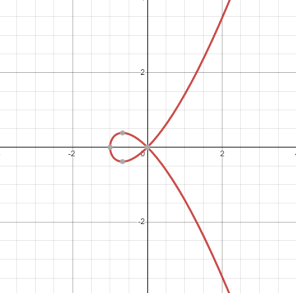
\includegraphics[scale=0.5]{graph1.png}

We often want to work over other fields such as
\(\mathbb{Q}, \mathbb{Z}/p\) where \(p\) is prime, etc. and a way to
understand their geometry is to look at their maximal ideals. In
\(\mathbb{C}\), it is much easier because by Hillbert's Nullstalensatz,
we know that in \(\mathbb{C}[x_1,x_2,\cdots,x_n]/(f)\) the maximal
ideals are of the form \((x_1-p_1,x_2-p_2,\cdots,x_n-p_n)\) where
\(f(p_1,\cdots,p_n)=0\)

The problem with other fields is that the maximal ideals are a
topological space, but the topology is too weak. By weak, we mean that
the neighborhoods of the topology are too big, making it inconvenient to
study them in depth. There is no perfect analogy of an \(\epsilon\)-ball
around the origin for such fields when taking similar quotient rings.

Maximal ideals of a polynomial ring of \(n\)-variables defined over an
algebraically closed field \(k\) correspond to points in \(k^n\). For
example, if we take a polynomial ring in two variables \(R=k[x,y]\)
where \(k\) is an algebraically closed field, then the maximal ideals of
\(R\) all look like \((x-a,y-b)\) where \(a,b \in k\). These maximal
ideals correspond to point on \(k^2\). This is very convenient, however
in the case of non-singular algebraic varieties, it is impossible to find
neighborhoods of every point that behaves like a euclidean neighborhood
or a point, in other words like \(k^n\).

As an example, when examining \(\mathbb{Z}/5[x,y]/(y-x^2)\), then we
notice that there is a finite complement topology on it which means that
open sets are complements of finitely many closed sets. Therefore it is
not a Hausdorff space. Hausdorff spaces are much nicer to work with in
general, so this scenario will give us more difficulties.

\hypertarget{ring-completions}{%
\subsection{Ring Completions}\label{ring-completions}}

To avoid the difficulties, we have a solution called \emph{completion},
where instead we can choose a point in the algebraic variety which
corresponds to some maximal ideal in some ring. Then by
\emph{completing} the ring at the maximal ideal, we will always get
\(k[[x_1,\cdots,x_n]]\) which essentially replaces the neighborhood
concept we were looking for in a lot of cases, which is true by the
Cohen-Structure theorem. Vaguely speaking, power series rings can work
like ``small'' euclidean neighborhoods of a point on an algebraic
variety (the zero set of a multi-variable polynomial over a field).\cite{atiyah1994introduction} The
idea behind is that we are going to look at higher tangent information
instead of neighborhoods. Two polynomials are close to each other when
they agree in small degree. Then a sequence of polynomials \((f_i)\) is
Cauchy if for every \(\epsilon\) we can find \(N\in \mathbb{N}\) such
that for \(n,m > N\) then polynomials \(f_{n}\) and \(f_{m}\) agree in
degree less than or equal to \(\epsilon\). The objects of the completion
of a polynomial ring are equivalent classes of Cauchy sequences. Then
equivalence classes of Cauchy sequences are the same as formal power
series. This is analogous to set completions in analysis, however here
it is much generalized and is used in the same realm as localization.

    \hypertarget{lazy-power-series-package}{%
\section{Lazy Power Series package}\label{lazy-power-series-package}}

Our package makes it possible to work with formal power series, by
specifically introducing an object in Macaulay2 called
\texttt{LazySeries}. The reasoning behind the name is the construction
of the objects, as one of the main constructors is used by inputting an
explicit map that outputs the coefficients at any exponent given. This
is sort of a ``lazy'' way of dealing with power series, or rather a
generating function approach to it.

    \begin{tcolorbox}[breakable, size=fbox, boxrule=1pt, pad at break*=1mm,colback=cellbackground, colframe=cellborder]
\prompt{In}{incolor}{1}{\boxspacing}
\begin{Verbatim}[commandchars=\\\{\}]
loadPackage \PYZdq{}LazyPowerSeries\PYZdq{}
\end{Verbatim}
\end{tcolorbox}

    \begin{Verbatim}[commandchars=\\\{\}]

o1 = LazyPowerSeries

o1 : Package
    \end{Verbatim}

    \hypertarget{constructing-lazyseries}{%
\subsection{Constructing LazySeries}\label{constructing-lazyseries}}

Most series have enough information to extend their polynomial
approximation to arbitrary degree when needed. This means that even
though sums and products of series will return finite-precision results,
the precision can be increased at any time. Some of the ways you can
construct LazySeries for now are:

\begin{enumerate}
\def\labelenumi{\arabic{enumi}.}
\tightlist
\item
  Creating LazySeries by the \texttt{lazySeries(Ring,\ Function)} by
  using a given ring and function.
\item
  Creating LazySeries by the \texttt{lazySeries(RingElement)} by using a
  given ringElement.
\end{enumerate}

    \begin{tcolorbox}[breakable, size=fbox, boxrule=1pt, pad at break*=1mm,colback=cellbackground, colframe=cellborder]
\prompt{In}{incolor}{4}{\boxspacing}
\begin{Verbatim}[commandchars=\\\{\}]
R = ZZ[x]
f = i\PYZhy{}\PYZgt{} i
L = lazySeries(R, f)
\end{Verbatim}
\end{tcolorbox}

    \begin{Verbatim}[commandchars=\\\{\}]

           2     3
o4 = x + 2x  + 3x  + {\ldots}

o4 : LazySeries
    \end{Verbatim}

    \begin{tcolorbox}[breakable, size=fbox, boxrule=1pt, pad at break*=1mm,colback=cellbackground, colframe=cellborder]
\prompt{In}{incolor}{7}{\boxspacing}
\begin{Verbatim}[commandchars=\\\{\}]
R = ZZ[x]
p = x\PYZca{}5+765*x\PYZca{}4\PYZhy{}98*x\PYZca{}3+7

L = lazySeries(p)
\end{Verbatim}
\end{tcolorbox}

    \begin{Verbatim}[commandchars=\\\{\}]

            3
o7 = 7 - 98x  + {\ldots}

o7 : LazySeries
    \end{Verbatim}

    \hypertarget{changing-degrees}{%
\subsection{Changing degrees}\label{changing-degrees}}

The default degree of a LazySeries is 3. We can change the degree of a
LazySeries object by using the \texttt{changeDegree} after having
already created an object, or you could also change degree by specifying
the optional arguments \texttt{DisplayedDegree} and
\texttt{ComputedDegree} during initial construction by using options.
For now, we are using total degree, but we are planning on making it
possible to work with graded rings. You can right now, but it will take
the sum of the degree if you give it a list instead.

    \begin{tcolorbox}[breakable, size=fbox, boxrule=1pt, pad at break*=1mm,colback=cellbackground, colframe=cellborder]
\prompt{In}{incolor}{8}{\boxspacing}
\begin{Verbatim}[commandchars=\\\{\}]
changeDegree(L, 7)
\end{Verbatim}
\end{tcolorbox}

    \begin{Verbatim}[commandchars=\\\{\}]

            3       4    5
o8 = 7 - 98x  + 765x  + x  + {\ldots}

o8 : LazySeries
    \end{Verbatim}

    \begin{tcolorbox}[breakable, size=fbox, boxrule=1pt, pad at break*=1mm,colback=cellbackground, colframe=cellborder]
\prompt{In}{incolor}{9}{\boxspacing}
\begin{Verbatim}[commandchars=\\\{\}]
changeDegree(L, 2)
\end{Verbatim}
\end{tcolorbox}

    \begin{Verbatim}[commandchars=\\\{\}]

o9 = 7 + {\ldots}

o9 : LazySeries
    \end{Verbatim}

    \begin{tcolorbox}[breakable, size=fbox, boxrule=1pt, pad at break*=1mm,colback=cellbackground, colframe=cellborder]
\prompt{In}{incolor}{11}{\boxspacing}
\begin{Verbatim}[commandchars=\\\{\}]
f = i\PYZhy{}\PYZgt{} i\PYZca{}2
L = lazySeries(R, f, DisplayedDegree =\PYZgt{} 15, ComputedDegree =\PYZgt{} 15)
\end{Verbatim}
\end{tcolorbox}

    \begin{Verbatim}[commandchars=\\\{\}]

            2     3      4      5      6      7      8      9       10       11
12       13       14       15
o11 = x + 4x  + 9x  + 16x  + 25x  + 36x  + 49x  + 64x  + 81x  + 100x   + 121x
+ 144x   + 169x   + 196x   + 225x   + {\ldots}

o11 : LazySeries
    \end{Verbatim}

    \hypertarget{extracting-coefficients}{%
\subsection{Extracting coefficients}\label{extracting-coefficients}}

Sometimes it is convenient to just grab specific coefficients you are
looking for and there is a fast way to do it in this package by using
\texttt{coefficient} method.

    \begin{tcolorbox}[breakable, size=fbox, boxrule=1pt, pad at break*=1mm,colback=cellbackground, colframe=cellborder]
\prompt{In}{incolor}{12}{\boxspacing}
\begin{Verbatim}[commandchars=\\\{\}]
coefficient(\PYZob{}9\PYZcb{}, L)
\end{Verbatim}
\end{tcolorbox}

    \begin{Verbatim}[commandchars=\\\{\}]

o12 = 81
    \end{Verbatim}

    \begin{tcolorbox}[breakable, size=fbox, boxrule=1pt, pad at break*=1mm,colback=cellbackground, colframe=cellborder]
\prompt{In}{incolor}{13}{\boxspacing}
\begin{Verbatim}[commandchars=\\\{\}]
coefficient(\PYZob{}25\PYZcb{}, L)
\end{Verbatim}
\end{tcolorbox}

    \begin{Verbatim}[commandchars=\\\{\}]

o13 = 625

o13 : R
    \end{Verbatim}

    \hypertarget{multi-variable-rings}{%
\subsection{Multi-variable Rings}\label{multi-variable-rings}}

LazySeries construction works with multi-variable rings as well, as long
as the user inputs the function correctly. The function has to have the
same amount of inputs as the given ring variables. Here for example,
because we are given a polynomial ring of three variables over the
rationals, the function inputted takes three inputs (i,j,k). Another way
to input a function would be to make it take in a list that you are
assuming has the same amount of elements as the variables and sending it
to those values. Essentially, we are ensuring the function gives us a
coefficient based on the exponents.

    \begin{tcolorbox}[breakable, size=fbox, boxrule=1pt, pad at break*=1mm,colback=cellbackground, colframe=cellborder]
\prompt{In}{incolor}{16}{\boxspacing}
\begin{Verbatim}[commandchars=\\\{\}]
R = QQ[x,y,z]
f = (i,j,k)\PYZhy{}\PYZgt{} i+j+k+5

L = lazySeries(R, f)
\end{Verbatim}
\end{tcolorbox}

    \begin{Verbatim}[commandchars=\\\{\}]

                           2                   2            2     3       2
2     2               2      3       2     2      3
o16 = 5 + 6z + 6y + 6x + 7z  + 7y*z + 7x*z + 7y  + 7x*y + 7x  + 8z  + 8y*z  +
8x*z  + 8y z + 8x*y*z + 8x z + 8y  + 8x*y  + 8x y + 8x  + {\ldots}

o16 : LazySeries
    \end{Verbatim}

    \begin{tcolorbox}[breakable, size=fbox, boxrule=1pt, pad at break*=1mm,colback=cellbackground, colframe=cellborder]
\prompt{In}{incolor}{19}{\boxspacing}
\begin{Verbatim}[commandchars=\\\{\}]
R = ZZ/5[x,y,z]
f = (i,j,k)\PYZhy{}\PYZgt{} 8

L = lazySeries(R, f)
\end{Verbatim}
\end{tcolorbox}

    \begin{Verbatim}[commandchars=\\\{\}]

                            2                   2            2     3       2
2     2               2      3       2     2      3
o19 = -2 - 2z - 2y - 2x - 2z  - 2y*z - 2x*z - 2y  - 2x*y - 2x  - 2z  - 2y*z  -
2x*z  - 2y z - 2x*y*z - 2x z - 2y  - 2x*y  - 2x y - 2x  + {\ldots}

o19 : LazySeries
    \end{Verbatim}

    \hypertarget{addition}{%
\subsection{Addition}\label{addition}}

You can add two LazySeries together and it creates a new lazySeries with
its own unique function. This means that if you want to expand it, you
would be able to by changing its degree normally. Of course,
substraction works as well.

    \begin{tcolorbox}[breakable, size=fbox, boxrule=1pt, pad at break*=1mm,colback=cellbackground, colframe=cellborder]
\prompt{In}{incolor}{21}{\boxspacing}
\begin{Verbatim}[commandchars=\\\{\}]
R = ZZ[x,y]
L = lazySeries(R, (i,j)\PYZhy{}\PYZgt{}i)
\end{Verbatim}
\end{tcolorbox}

    \begin{Verbatim}[commandchars=\\\{\}]

                  2      2     2      3
o21 = x + x*y + 2x  + x*y  + 2x y + 3x  + {\ldots}

o21 : LazySeries
    \end{Verbatim}

    \begin{tcolorbox}[breakable, size=fbox, boxrule=1pt, pad at break*=1mm,colback=cellbackground, colframe=cellborder]
\prompt{In}{incolor}{22}{\boxspacing}
\begin{Verbatim}[commandchars=\\\{\}]
M = lazySeries(R, (i,j)\PYZhy{}\PYZgt{}j)
\end{Verbatim}
\end{tcolorbox}

    \begin{Verbatim}[commandchars=\\\{\}]

            2           3       2    2
o22 = y + 2y  + x*y + 3y  + 2x*y  + x y + {\ldots}

o22 : LazySeries
    \end{Verbatim}

    \begin{tcolorbox}[breakable, size=fbox, boxrule=1pt, pad at break*=1mm,colback=cellbackground, colframe=cellborder]
\prompt{In}{incolor}{23}{\boxspacing}
\begin{Verbatim}[commandchars=\\\{\}]
S = L+M
\end{Verbatim}
\end{tcolorbox}

    \begin{Verbatim}[commandchars=\\\{\}]

                2            2     3       2     2      3
o23 = y + x + 2y  + 2x*y + 2x  + 3y  + 3x*y  + 3x y + 3x  + {\ldots}

o23 : LazySeries
    \end{Verbatim}

    \begin{tcolorbox}[breakable, size=fbox, boxrule=1pt, pad at break*=1mm,colback=cellbackground, colframe=cellborder]
\prompt{In}{incolor}{24}{\boxspacing}
\begin{Verbatim}[commandchars=\\\{\}]
changeDegree(S, 4)
\end{Verbatim}
\end{tcolorbox}

    \begin{Verbatim}[commandchars=\\\{\}]

                2            2     3       2     2      3     4       3     2 2
3      4
o24 = y + x + 2y  + 2x*y + 2x  + 3y  + 3x*y  + 3x y + 3x  + 4y  + 4x*y  + 4x y
+ 4x y + 4x  + {\ldots}

o24 : LazySeries
    \end{Verbatim}

    \begin{tcolorbox}[breakable, size=fbox, boxrule=1pt, pad at break*=1mm,colback=cellbackground, colframe=cellborder]
\prompt{In}{incolor}{25}{\boxspacing}
\begin{Verbatim}[commandchars=\\\{\}]
S = L\PYZhy{}M
\end{Verbatim}
\end{tcolorbox}

    \begin{Verbatim}[commandchars=\\\{\}]

                 2     2     3      2    2      3
o25 = -y + x - 2y  + 2x  - 3y  - x*y  + x y + 3x  + {\ldots}

o25 : LazySeries
    \end{Verbatim}

    \hypertarget{multiplication}{%
\subsection{Multiplication}\label{multiplication}}

One of the concerns for multiplication was speed, but so far it is fast
enough. Additionally, we have a more efficient way of calculating powers
of LazySeries objects by using exponentiating by squaring method, also
known as double-and-add method which uses binary conversion of a power
to determine the steps it needs to take to calculate up to that certain
power in fewer steps than it would take to primitively multiply that
many times. It reduces the amount of steps it would take with the
primitive approach, but of course this is an open problem and does not
always guarantee the fastest way of calculating the powers.

    \begin{tcolorbox}[breakable, size=fbox, boxrule=1pt, pad at break*=1mm,colback=cellbackground, colframe=cellborder]
\prompt{In}{incolor}{29}{\boxspacing}
\begin{Verbatim}[commandchars=\\\{\}]
R = ZZ[x,y]

L = lazySeries(R, (i,j)\PYZhy{}\PYZgt{}1+i)
M = lazySeries(R, (i,j)\PYZhy{}\PYZgt{}j)
L*M
\end{Verbatim}
\end{tcolorbox}

    \begin{Verbatim}[commandchars=\\\{\}]

            2            3       2     2
o29 = y + 3y  + 3x*y + 6y  + 9x*y  + 6x y + {\ldots}

o29 : LazySeries
    \end{Verbatim}

    \begin{tcolorbox}[breakable, size=fbox, boxrule=1pt, pad at break*=1mm,colback=cellbackground, colframe=cellborder]
\prompt{In}{incolor}{30}{\boxspacing}
\begin{Verbatim}[commandchars=\\\{\}]
L\PYZca{}2
\end{Verbatim}
\end{tcolorbox}

    \begin{Verbatim}[commandchars=\\\{\}]

                      2             2     3        2      2       3
o30 = 1 + 2y + 4x + 3y  + 8x*y + 10x  + 4y  + 12x*y  + 20x y + 20x  + {\ldots}

o30 : LazySeries
    \end{Verbatim}

    \begin{tcolorbox}[breakable, size=fbox, boxrule=1pt, pad at break*=1mm,colback=cellbackground, colframe=cellborder]
\prompt{In}{incolor}{31}{\boxspacing}
\begin{Verbatim}[commandchars=\\\{\}]
L\PYZca{}10
\end{Verbatim}
\end{tcolorbox}

    \begin{Verbatim}[commandchars=\\\{\}]

                         2                2       3          2        2
3
o31 = 1 + 10y + 20x + 55y  + 200x*y + 210x  + 220y  + 1100x*y  + 2100x y + 1540x
+ {\ldots}

o31 : LazySeries
    \end{Verbatim}

    \hypertarget{inversion}{%
\subsection{Inversion}\label{inversion}}

For inversion, first of all the formal power series has to be invertible
and that can be checked if its constant term is invertible in the given
ring. We use the formula \((1-x)^{-1} = 1+x+x^2+x^3+...\), which is
valid with formal power series as well. The algorithm of our inversion
function works like so (it is easier to see in one-variable case but you
can expand it to multi0variable just as easily): First we are given a
LazySeries L that has the form \[a_0+a_1x+a_2x^2+\cdots\]. We want to
make it look like the initial formula we showed, therefore we take out
the constant term and separate it from 1 to look like so:
\[a_0(1+\frac{a_1}{a_0}x+\frac{a_2}{a_0}x^2 +\cdots)\]
\[a_0(1-(-\frac{a_1}{a_0}x-\frac{a_2}{a_0}x^2 -\cdots))\] We can just
denote \(g := (-\frac{a_1}{a_0}x-\frac{a_2}{a_0}x^2 -\cdots)\) and we
have \[a_0(1-g) \] If we invert it, then
\[(a_0(1-g))^{-1} = \frac{1}{a_0}(1+g+g^2+g^3+\cdots) \]

    \begin{tcolorbox}[breakable, size=fbox, boxrule=1pt, pad at break*=1mm,colback=cellbackground, colframe=cellborder]
\prompt{In}{incolor}{33}{\boxspacing}
\begin{Verbatim}[commandchars=\\\{\}]
R = ZZ[x,y]
L = lazySeries(R, (i,j)\PYZhy{}\PYZgt{} 1 + i)
\end{Verbatim}
\end{tcolorbox}

    \begin{Verbatim}[commandchars=\\\{\}]

                    2            2    3       2     2      3
o33 = 1 + y + 2x + y  + 2x*y + 3x  + y  + 2x*y  + 3x y + 4x  + {\ldots}

o33 : LazySeries
    \end{Verbatim}

    \begin{tcolorbox}[breakable, size=fbox, boxrule=1pt, pad at break*=1mm,colback=cellbackground, colframe=cellborder]
\prompt{In}{incolor}{34}{\boxspacing}
\begin{Verbatim}[commandchars=\\\{\}]
inverseL = inverse(L)
\end{Verbatim}
\end{tcolorbox}

    \begin{Verbatim}[commandchars=\\\{\}]

                           2    2
o34 = 1 - y - 2x + 2x*y + x  - x y + {\ldots}

o34 : LazySeries
    \end{Verbatim}

    \begin{tcolorbox}[breakable, size=fbox, boxrule=1pt, pad at break*=1mm,colback=cellbackground, colframe=cellborder]
\prompt{In}{incolor}{35}{\boxspacing}
\begin{Verbatim}[commandchars=\\\{\}]
L*inverseL
\end{Verbatim}
\end{tcolorbox}

    \begin{Verbatim}[commandchars=\\\{\}]

o35 = 1 + {\ldots}

o35 : LazySeries
    \end{Verbatim}

    \hypertarget{some-additional-methods}{%
\subsection{Some additional methods}\label{some-additional-methods}}

\texttt{sub} is a method that promotes LazySeries objects of a specified
ring to a new ring, essentially promoting each term to a polynomial in
the ring. \texttt{isUnit} is a very useful tool to check if a LazySeries
object is invertible by checking if the constant term is invertible in
the specified ring.

    \begin{tcolorbox}[breakable, size=fbox, boxrule=1pt, pad at break*=1mm,colback=cellbackground, colframe=cellborder]
\prompt{In}{incolor}{38}{\boxspacing}
\begin{Verbatim}[commandchars=\\\{\}]
R = ZZ[x,y]
L = lazySeries(R, (i,j)\PYZhy{}\PYZgt{} 1 + i)
S = QQ[x,y]
\end{Verbatim}
\end{tcolorbox}

    \begin{Verbatim}[commandchars=\\\{\}]

o38 = S

o38 : PolynomialRing
    \end{Verbatim}

    \begin{tcolorbox}[breakable, size=fbox, boxrule=1pt, pad at break*=1mm,colback=cellbackground, colframe=cellborder]
\prompt{In}{incolor}{39}{\boxspacing}
\begin{Verbatim}[commandchars=\\\{\}]
newL = sub(L, S)
\end{Verbatim}
\end{tcolorbox}

    \begin{Verbatim}[commandchars=\\\{\}]

                    2            2    3       2     2      3
o39 = 1 + y + 2x + y  + 2x*y + 3x  + y  + 2x*y  + 3x y + 4x  + {\ldots}

o39 : LazySeries
    \end{Verbatim}

    \begin{tcolorbox}[breakable, size=fbox, boxrule=1pt, pad at break*=1mm,colback=cellbackground, colframe=cellborder]
\prompt{In}{incolor}{40}{\boxspacing}
\begin{Verbatim}[commandchars=\\\{\}]
class newL.cache.displayedPolynomial
\end{Verbatim}
\end{tcolorbox}

    \begin{Verbatim}[commandchars=\\\{\}]

o40 = S

o40 : PolynomialRing
    \end{Verbatim}

    \begin{tcolorbox}[breakable, size=fbox, boxrule=1pt, pad at break*=1mm,colback=cellbackground, colframe=cellborder]
\prompt{In}{incolor}{41}{\boxspacing}
\begin{Verbatim}[commandchars=\\\{\}]
isUnit(L)
\end{Verbatim}
\end{tcolorbox}

    \begin{Verbatim}[commandchars=\\\{\}]

o41 = true
    \end{Verbatim}

    \begin{tcolorbox}[breakable, size=fbox, boxrule=1pt, pad at break*=1mm,colback=cellbackground, colframe=cellborder]
\prompt{In}{incolor}{42}{\boxspacing}
\begin{Verbatim}[commandchars=\\\{\}]
M = lazySeries(R, (i,j)\PYZhy{}\PYZgt{}i)
\end{Verbatim}
\end{tcolorbox}

    \begin{Verbatim}[commandchars=\\\{\}]

                  2      2     2      3
o42 = x + x*y + 2x  + x*y  + 2x y + 3x  + {\ldots}

o42 : LazySeries
    \end{Verbatim}

    \begin{tcolorbox}[breakable, size=fbox, boxrule=1pt, pad at break*=1mm,colback=cellbackground, colframe=cellborder]
\prompt{In}{incolor}{43}{\boxspacing}
\begin{Verbatim}[commandchars=\\\{\}]
isUnit(M)
\end{Verbatim}
\end{tcolorbox}

    \begin{Verbatim}[commandchars=\\\{\}]

o43 = false
    \end{Verbatim}

    \hypertarget{future-goals-for-the-package}{%
\section{Future goals for the
package}\label{future-goals-for-the-package}}

The next steps of this project is to expand on our implementation of
power series element as an object in Macaulay2 and to build on the
object of a ring to make a power series ring subclass. We plan to add
more functionality, such as adding more types of constructors, as well
as making sure the package works with multi-graded rings. Additionally,
we will introduce quotient rings, ideals and modules over a power
series, while also making it possible to complete a polynomial ring at a
maximal ideal to get a power series ring. We are also interested in
exploring the field of \(p\)-adic numbers \(\mathbb{Q}_p\) where \(p\)
is a prime integer.

    % Add a bibliography block to the postdoc
\bibliographystyle{plain}
\bibliography{bibliography.bib}
    

\end{document}
